
\chapter{\textsc{Modélisation du système Segment Piston Chemise (SPC)} }
\lettrine{L}{a} compréhension du comportement des surfaces en contact dans les système \emph{SPC}, a une importance capitale dans l'amélioration de performance du moteur à combustion interne. La lubrification qui se produit dans l'interface \emph{SPC} impose une certaine forme assez particulière de mode de lubrification qui couvre le régime mixte, hydrodynamique et critique. Ainsi pour la représentation mathématique de ce système physique, doit prendre en considération chaque mode de lubrification que nous allons développer dans la suite.
\section{CARACTERISATION DE LA TOPOGRAPHIE  DE LA CHEMISE}

\lettrine{L}{a} prise en compte de la caractérisation de la surface, influence en grande partie sur les performances du moteur. celle-ci influence la qualité de la séparation du contact mais aussi le transport du lubrifiant par les segments le long de la chemise. Dans la suite. Gardons à l'esprit que la prise en compte des effets de la rugosité en lubrification des corps en mouvement relatif, est un problème assez compliqué faisant intervenir de nombreux aspect; entre autre le caractère changeant du domaine occupé par le fluide en mouvement relatif, ou la déformation de surface de corps en mouvement relatif. En outre les difficultés liées à la physique des fluides, qui peut être plus ou moins complexe suivant les cas ou la nature du lubrifiant : effets de compressibilité, effets piézovisqueux, cavitation, couplage avec la thermique pour ne cité que çà. Aussi, une autre difficulté est liée à la difference nette entre l'échelle de grandeur de la rugosité et celle de l'ingénieur qui est généralement de de plusieurs ordres de grandeur plus grandes que celle de la rugosité (généralement inférieur à $0.001$ )\cite{initiation}\\

Quelque soit le moyen de mise en oeuvre utilisé, les surfaces présentent des écarts
géométriques par rapport à leur forme théorique.Ces défauts jouent un rôle primordial en tribologie. On peut classer les défauts en fonction de leur longueurs d’onde $L$ Image \ref{fig:ondulation}  \cite{initiation} :
\begin{itemize}
	\item si $L$ est de l’ordre de la taille de la surface, on parle de défaut de forme ;
	\item Lorsque $0.001m < L < 0.01m$, on parle de defaut d'ondulation;
	\item les défauts de longueur d’onde inférieur sont appelés rugosité.
\end{itemize}
% TODO: \usepackage{graphicx} required
\begin{figure}
	\centering
	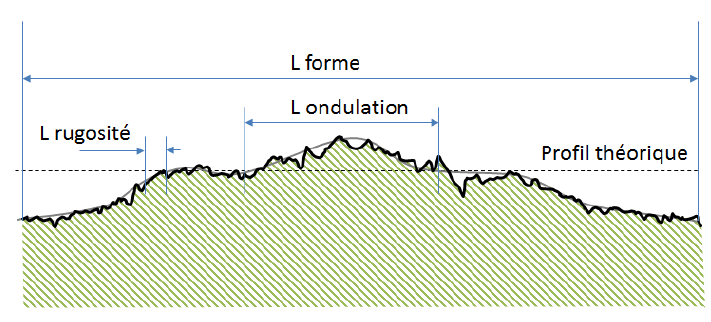
\includegraphics[width=0.7\linewidth]{Img/ondulation}
	\caption[Défaut géométrique du surfacee]{Défaut géométrique du surface}
	\label{fig:ondulation}
\end{figure}
La rugosité est donc l'ensemble des irrégularités microscopique et macroscopique d'une surface.
Toutes les surfaces, naturel ou fabriqué, ne sont pas parfaitement lisses. La surface la plus
douce dans les corps normaux est celle du \emph{mica}. Le \emph{mica} a une rugosité approximativement de $0.002032 microns$.\cite{ayad1}
\subsection{Méthodes des texturation des chemises}
\lettrine{L}{a} majeur partie des pièces de moteur vient de l'industrie métallurgique. Dans leur proceder de fabrication plusieur méthodes de finissage de la surface sont employées. Le principale étant l'abrasion par \emph{galetage} \footnote{Techniquqe de finissage  de la surface qui peut avoir plusieurs objectifs comme le renforcement mécanique de la surface} et \emph{ grenaillage} \footnote{c'est une technique qui consiste à projeter à grande vitesse des billes sur la surface d'un objet pour en modifier la structure superficielle, a fin d'améliorer l'aspect et les caractéristiques techniques.} sont les premières opérations qui vont permettre une maîtrise de rugosité jusqu’à un ordre de grandeur de 0.5mm.\cite{ayad1} À partir de l’état de surface obtenu, on cherchera à introduire une "texturation" qui va permettre de créer une rugosité plus "précise" sur l’interface de la surface Image \ref{fig:caracterisation}.
% TODO: \usepackage{graphicx} required
\begin{figure}[h]
	\centering
	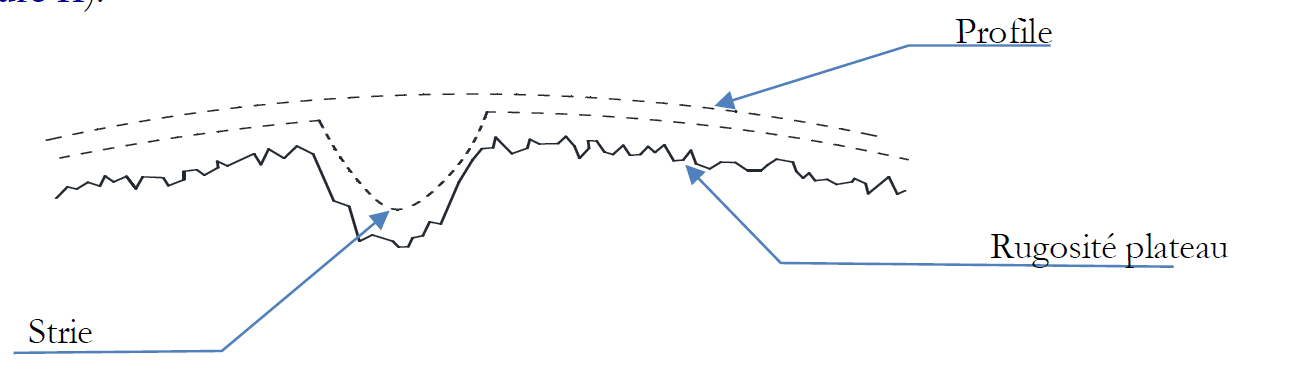
\includegraphics[width=0.7\linewidth]{Img/caracterisation}
	\caption[surface texturée]{Profil de rugosité de surface texturée}
	\label{fig:caracterisation}
\end{figure}
\subsubsection{Texturation avec procédé chimique}
\lettrine{D}{ans} cette technique, un film protecteur est posé sur la surface de la pièce. Ce film est muni de motif par lequel un acide va s’infiltrer pour attaquer l’interface. La concentration utilisée et le temps laissé avant le rinçage déterminent la profondeur de la texture souhaitée. Cette technique a l’avantage de ne pas entraîner de déformation du matériau autour de la texture, de ne pas générer de débris pouvant subsister dans le contact, mais elle est très lourde à mettre en place sur une chaîne de production, car il faut isoler toutes les parties qui ne seront pas concernés par la texturation.
\subsubsection{Texturation à l'aide d'un diamant}
\lettrine{D}{ans} ce procédé d’usinage, un diamant est utilisé pour réaliser la texturation, 3 paramètres permettent de contrôler la texture obtenue :
\begin{itemize}	
	\item La vitesse de deplacement verticale;
	\item La vitesse de rotation du rodoir;
	\item La vitesse d'abrasion des diamants.
\end{itemize}
Ce procédé a plusieurs avantages : rapidité, bonne finition, peu coûteux, facile à mettre en place sur les chaînes de production, mais la surface s’en trouve légèrement déformée autour de la texture.

\subsection{Paramètres de rugosités}
\lettrine{L}{e} Tout premier appareil de mesure du profil de la surface est le palpeur en diamant. Cette appareil se deplace longitidalement sur la face en donnant généralement un ensemble des points $n$ de variation de la hauteur $z_i$ espacé d'une intervalle latéral $\delta x$. A partir de cette série, on peut calculer des paramètres d’amplitude. Le plus utilisé dans la communauté des mécaniciens est le $R_a$ \cite{initiation}. Pendans longtemps un seul paramètre était connu et utilisé $R_a$ (Routhness Average), d'autres paramètres sont venus après comme RMS(Rout Mean Squart). Aujourd'hui, les paramètres de mesure de surface sont définis suivant plusieurs normes internationales où il y a même des variantes sectorielles (la sidérurgie ou l'automobile). On distingue trois groupes de paramètres de mesure utilisés selon le type de profil \cite{ayad1}:
\begin{itemize}
	\item Paramètres de préfixe P calculés sur le \textbf{profil primaire};
	\item Paramètres de préfixe R calculés sur le \textbf{profil de rugosité} ;
	\item Paramètres de préfixe W calculés sur le \textbf{profil d'ondulation}.
\end{itemize}
Dans le cadre notre travail; nous allons être indulgent envers nous-même en limitant notre travail dans l'étude de la surface  par le préfixe de R du \emph{profil de rugosité} pour simplifier le travail.\\

La figure \ref{fig:profil-surface} présente un exemple de profil de surface. L’échelle verticale est amplifiée par rapport à l’échelle horizontale pour que les rugosités puissent être discernées.En coupant le profil par une ligne horizontale, il est possible de calculer le pourcentage de points situés au dessus de la ligne. En balayant verticalement le profil avec la ligne horizontale, on obtient l’évolution de ce pourcentage en fonction de la hauteur $z$. La courbe obtenu est appelée \emph{courbe de portance} ou \emph{courbe d'Abbott} (Figure \ref{fig:analysedistribution}). Elle indique le pourcentage de points qui entrerait en contact avec un plan rigide situé à la hauteur $z$.\cite{initiation}
% TODO: \usepackage{graphicx} required
\begin{figure}[h]
	\centering
	\includegraphics[width=0.7\linewidth]{"Img/profil surface"}
	\caption[profil surface]{Profil de surface}
	\label{fig:profil-surface}
\end{figure}
% TODO: \usepackage{graphicx} required
\begin{figure}[h]
	\centering
	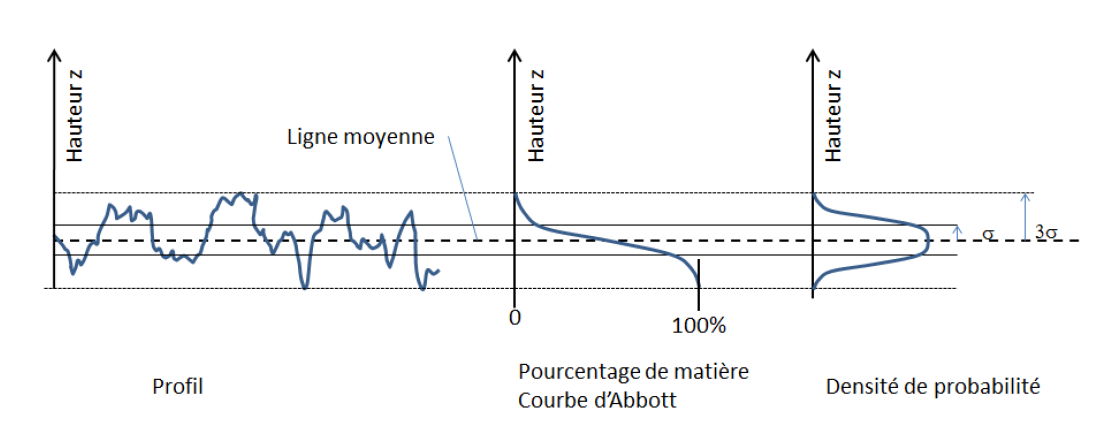
\includegraphics[width=0.7\linewidth]{Img/analysedistribution}
	\caption[analyseRigosité]{Analyse de rigosité}
	\label{fig:analysedistribution}
\end{figure}

Les paramètres d’évaluation de la topographie d’une surface sont référencés par une lettre majuscule R indicé d’une lettre minuscule propre au paramètre. Dans le soucis de la préservation de la tradition du métier de mécanicien, nous allons garder la même notation :
\begin{equation}
	{R}_{a}=\frac{1}{n}\sum _{1}^{n}\left|z_i\right|
	\label{Ra}
\end{equation}
\begin{equation}
	{R}_{a}=\frac{1}{L}{\int }_{0}^{L}\left|z\right|dx
\end{equation}
On utilise également $R_q$ ou RMS:
\begin{equation}
		{R}_{q}=\sqrt{\frac{1}{n}\sum _{1}^{a}{z_i}^{2}}
\end{equation}
\begin{equation}
		{R}_{q}=\sqrt{\frac{1}{L}{\int }_{0}^{L}{z}^{2}}
\end{equation}

Ce paramètre $R_q$ est équivalent à l’écart type, on utilisons aussi un paramètre de symétrie
\begin{equation}
	RSk=\frac{1}{n{R}_{q}^{3}}\sum {z}_{i}^{3}
\end{equation}
\begin{equation}
	RSk=\frac{1}{L{R}_{q}^{3}}\underset{0}{\int }{z}^{3}\left(x\right)dx
\end{equation}
Une valeur positive de ce paramètre indique des pics plus marqués que les vallées. La
situation inverse correspond à une valeur négative de $RSk$. Enfin, le paramètre d’étalement
indique sur quelle étendue sont distribués les points de la surface :
\begin{equation}
	RKu=\frac{1}{n{R_q}^{4}}\Sigma {z}_{i}^{4}
\end{equation}
\begin{equation}
	RKu=\frac{1}{L{R_q}^{4}}\int_{0}^{L}{z}_{i}^{4}
\end{equation}
